\section{Introduction} \label{sec:intro}

Rubin Observatory Data Management conducted the second operations rehearsal (milestones LDM-503-11 see \citeds{LDM-503}) from July 28$^{th}$ to 30$^{th}$ 2020.
The plan for the rehearsal was outlined in \citeds{LDM-643}, the main principle was to simulate
nominal operations with ComCam calibration data flowing from Chile, being processed (calibrated)
and having some quality assurance performed.  The overall emphasis was to investigate/simulate how
raft-scale data can be acquired and processed in preparation for ComCam commissioning activities.
\citeds{LDM-643} details the procedure and personnel involved,
hence in this document we give a brief summary of what  happened in the rehearsal taking that as read.


\section{The rehearsal \#2}

There was a short preliminary meeting on the Monday (July 27$^{th}$ 2020), immediately prior to the
rehearsal start to ensure hardware, software, and personnel were ready.

\subsection{System Configuration During the Rehearsal} \label{sec:setup}

ComCam had been installed at the Base (La Serena) computer room and basic operation using the OCS/Archiver
mode had been enabled.  The hardware installation was a filter-less ComCam (with {\it r}-band hard coded
in headers) and basic functionality to obtain bias, flat, and dark frames.

Data transfer from the Base to the current USDF at NCSA were accomplished but the long-haul networks were not
fully operational.  The raft-scale data were ingested into Butler (gen2) repos on arrival at the USDF
and made available through the {\it \/project\/shared/comCam} space (also visible for the RSP).

Processing was accomplished using the nascent utilities processBias.py, processFlat.py, processDark.py
and ingestCalib.py.

The calibrations frames taken were bias, dark, flat sequences of roughly 10 exposures each on each night.
There exist extraneous exposures within the sets but the main calibration sequences used {\it groupId}'s
(e.g., CALSET\_20200728\_1920) to facilitate their identification.  Due to an upcoming quarantine in Chile
(due to COVID-19) the calibration sequences were obtained the evening prior to each "night" of the
rehearsal so that the rehearsal could be completed before the lock down began but also to hedge against
slow transfers (because the long-haul networks were not fully functional).  Processing occurred either
in the evening or morning after (depending on the transfer time) and analysis and QA occurred
shortly thereafter.

\subsubsection{Communications }


A Slack channel \href{https://lsstc.slack.com/messages/CJBSY6FUN}{\#ops-rehearal-2} was created to support communications.

A daily telecon was held using bluejeans at 10:00PST with the agenda:
\begin{itemize}
\item Observing: Recap of previous night's calibrations.
\item Data transfer summary:  How did data transfer and ingest go.
\item Pipeline Processing Summary: 	How did processing go.  Were there errors, incidents, caveats and reference to logs.
\item Metrics/QA:  What can we say about the data. Summary plots and metrics.  What is missing in our view. What can we add for next night?
\item Status:   Current instrument status.  Discuss current plans, changes, action items.

\end{itemize}


\subsection{Day 1} \label{sec:day1}

The daily meeting took place as planned at 11:00 PST.

Bias, Flat, and Dark sequences were acquired.  A clear problem, L3 fogging, was 
noted and resulted in the replacement of the N2 bottle.  It was noted that 
fogging was clearing and flats on subsequent nights should show a change.  

Transfers showed problems with roughly 25s per file (CCD).  The $\sim$30 exposure 
required O(1.5 hours) to reach the USDF.  On arrival problems were detected with
the ingestion of data.  The culprit was that two processes were trying to ingest 
incoming files (one linking them with a deprecated file path).  Once transfers 
completed, data repositories were regenerated fixing the issue.  

Processing proceeded rapidly.  Jobs were submitted using parallelism over 9 CCDs
making up the ComCam raft.  Total processing time was O(15 minutes) using 10 cores.
There were problems with calibration ingestion (the CALIB area does not have 
permissions to allow group access).  It is suspected that this has caused preliminary 
calibration based on early ComCam tests from a few week prior to be used in the 
reduction of the new calibration data but current provenance did not show
which calibraitons were used.

QA was performed with notebooks shared.  This analysis demonstrated that the 
proper calibrations were not used.  

\subsubsection{Discussion}
We discussed how to implement change in infrastructure to support the current
Butler Gen2 usage of calibrations (group write permissions were extended for the
interim).  Further discussions about Gen2 vs. Gen3 and the level of sophistication
to plan for the next rehearsal.  


\subsection{Day 2} \label{sec:day2}

The daily meeting took place as planned at 11:00 PST. \footnote{\url{https://confluence.lsstcorp.org/display/DM/OPS+Rehearsal+\%28Day+2\%3A+2020-07-29\%29+Meeting+notes}}

Initial data tests took O(2 hours).  Second test provided calibrations for the
second night (flats should not show condensation \figref{fig:d1}).

Transfers were again slow and DB access was not provided in monitoring scripts, so
timing relied on file creation times (fixes were added after the meeting).  LHN
staff are looking at slow transfer speeds.

Processing proceeded similar to the night before.  Provisional changes in
CALIB area permissions worked, but is still unclear how to see the logs.  One dark frame
had problems with only 6 of 9 files being transferred (required a restart).

Quality analyses showed a huge change in flat frames (confirming that
moisture indeed impacted previous calibrations \figref{fig:d1}).


\begin{figure}
\begin{center}
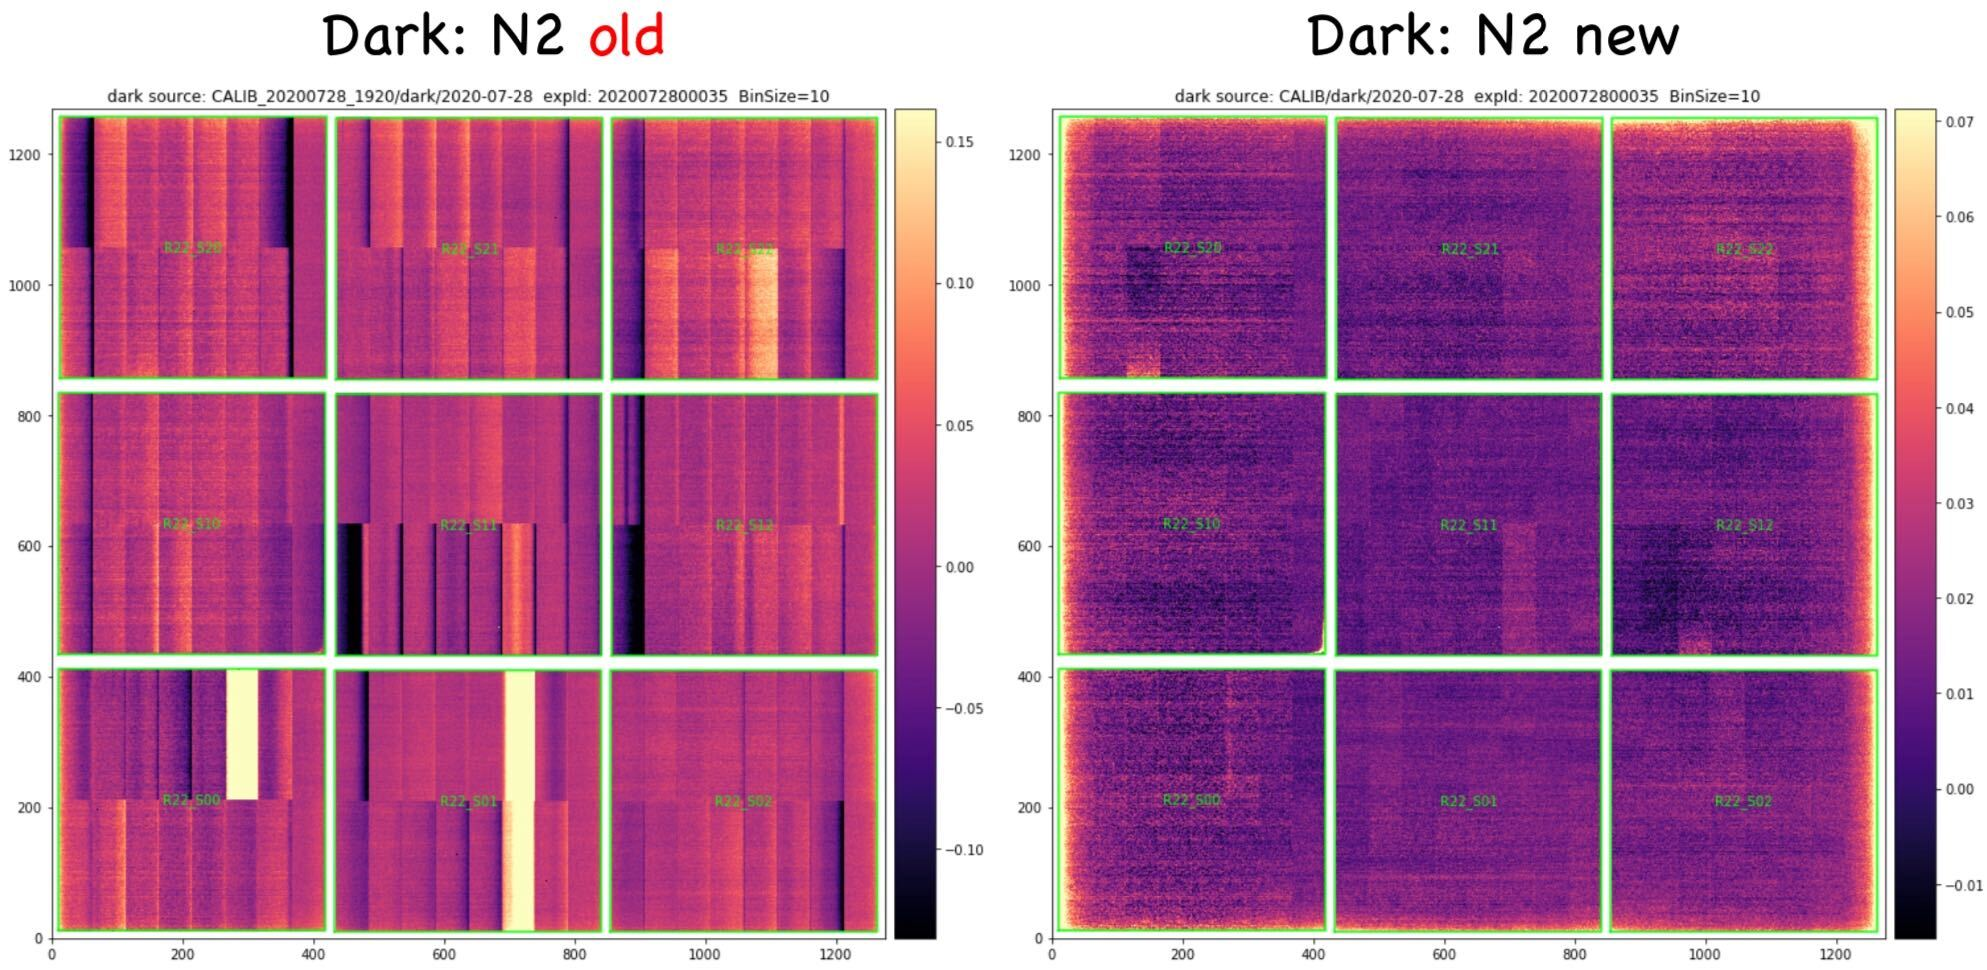
\includegraphics[width=0.9\textwidth]{figures/n2bad}
\end{center}
\caption{Left: Night 2 dark with incorrect bias subtracted.  Right: Night 2 dark with correct bias subtracted.\label{fig:d2}}
\end{figure}

\subsubsection{Discussion}

The plans for the next night were discussed.  Initially there were supposed to be
changes, with an aborted flat sequence followed by change in illumination prior to
the "real" sequence being taken.  This plan was altered in favor of attempting to
get some preliminary estimates about the overall stability of the instrument from
one night to the next while in its temporary (not so stable) environment.  So the
upcoming calibration sequences were planned to have no explicit changes.
The associated QA analysis revealed an instability in (at least) the bias frames \figref{fig:d3}



\subsection{Day 3} \label{sec:day3}

The daily meeting took place as planned at 11:00 PST.\footnote{\url{https://confluence.lsstcorp.org/display/DM/OPS+Rehearsal+\%28Day+3\%3A+2020-07-30\%29+Meeting+notes}}

Observations were attempted to repeat images with the previous night's setup.  There was a
disk write timeout from the DAQ.  This was mitigated, the exposure counter was incremented
and a restart allowed the completion of the sequences.  It was noted that this
problem will likely go away once SSDs are installed for the DAQ storage hardware.

Transfers required 2 hours, 50~s for the first image and then downhill from there.
Processing proceeded without incident and all calibrations went to the correct
registry.

Quality analyses show huge differences in darks between nights but this has been
traced to the wrong bias frames (those from 2 weeks prior) being applied.


\begin{figure}
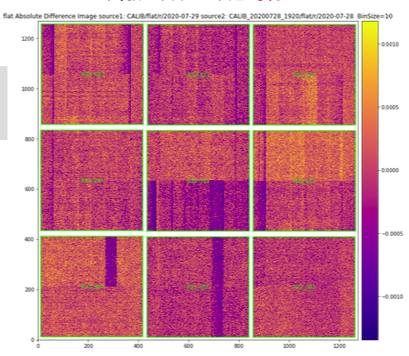
\includegraphics[width=0.45\textwidth]{figures/n3-2bad}
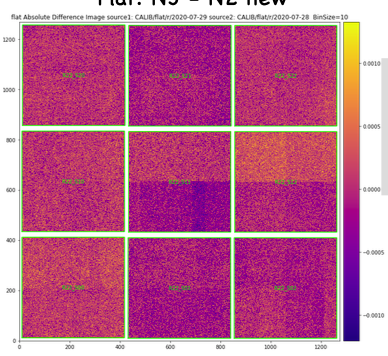
\includegraphics[width=0.43\textwidth]{figures/n3-2}
	\caption{Difference between night two and night three flats with incorrect bias(left),  correct bias subtraction (right).\label{fig:d3}}
\end{figure}


\subsubsection{Discussion}

The rehearsal was deemed finished, except for some follow-on analyses and
the production of this report.  Most discussion revolved around the soonest that
a subsequent rehearsal should be planned (even if it were to repeat this
exercise) and what changes we should plan for.  The current thought is that we
should begin discussing this in September and should set a goal to be able to
switch to using the Gen3 Butler and code-base (with high priority).






\section{Conclusion and lessons learned}\label{sec:conc}
This rehearsal was slightly delayed to allow us to use ComCam. Even though it was in the base facility and not on
the mountain it was still worth waiting for.
It is a less than ideal situation born out by the first images with moisture on the lens due to the N2 running out
and the poor long-haul network performance throughout (O(25 Mb/s) compared to the current expected 10 Gb/s and the
eventual planned 100 Gb/s).
The team in this rehearsal, using actual hardware, had a more active role for the $``$observing specialist on the mountain$''$ (in this case setting up the flat for the camera and initiating the observing sequence).
We used software from Telescope and Site, Camera and DM to take the images and transfer them to NCSA.
All of this activity underpinned by machines and networks supported by Rubin IT.
This is a first true demonstration of multiple parts of the system working together in an operational manner.
All of the hard integration efforts of SITCOM have born fruit for us here.

Among the lessons learned from this rehearsal are:
\begin{itemize}
\item We ran into networking problems and we were not easily able to diagnose them - we should have included key
long-haul network people in the rehearsal and we shall next time.

\item We encountered problems with Data Management pipeline configuration. Documentation and training need to be provided.

\item We still need to have automated processing in place for images - in the plan but not yet available.
\end{itemize}

In summary, this was a very good rehearsal the teams worked well together, there remains plenty to do in future rehearsals!





